 \documentclass[10pt,a4paper]{article}
\usepackage[utf8x]{inputenc}
\usepackage[danish]{babel}
\usepackage{amsmath}
\usepackage{mathtools}
\usepackage{framed}
\usepackage{amsfonts}
\usepackage{hyperref}
\usepackage{listings}
\usepackage{xcolor}
\lstset { %
    language=C++,
    backgroundcolor=\color{black!5}, % set backgroundcolor
    basicstyle=\footnotesize,% basic font setting
}
\usepackage{float}
\usepackage{amssymb}
\setlength{\parindent}{0pt}
\usepackage{graphicx}
\usepackage{fullpage}
\DeclarePairedDelimiter\ceil{\lceil}{\rceil}
\DeclarePairedDelimiter\floor{\lfloor}{\rfloor}
\newcount\colveccount
\newcommand*\colvec[1]{
        \global\colveccount#1
        \begin{pmatrix}
        \colvecnext
}
\def\colvecnext#1{
        #1
        \global\advance\colveccount-1
        \ifnum\colveccount>0
                \\
                \expandafter\colvecnext
        \else
                \end{pmatrix}
        \fi
}
\title{First Report - AI}
\date{\today}
\author{}
\begin{document}
\maketitle
\newpage
\textbf{ 1.  What behaviours or functions will you equip the robot with, so it can complete
     the Sokoban course successfully?}\\
     
     The robot is capable of turning left and right as well as moving forward. The robot is can perform these command based on the input file it provided with. The input file contains a string of the movement the robot has to perform in order the solve the sokoban game. \\
     
	A special function capable of moving the tin one step forward is  also implemented. In this function is each wheel rotated  with a specified amount of revolutions forward such that the tin will be moved to the next position. The robot will then using its sensor  move back to its original position. \\

     
     Besides its movement capabilities,  the robot also knows its orientation. This implementation was chosen in order to separate the functionality of the Sokoban solver and the movement of the robot.  The functionality of constantly knowing the orientation was considered more meaningful for the robot rather than the solver. 
     
\begin{lstlisting}
bool forward()
{    
    OnRev(MOTOR_LEFT,BASE_SPEED);
    OnRev(MOTOR_RIGHT,BASE_SPEED); 
    Wait(300); 
    sensor_line_input = GetInput(SENSOR_LINE,RawValueField);
    while(CROSS_THRESHOLD > sensor_line_input)
    {
        sensor_right_input = GetInput(SENSOR_RIGHT,RawValueField);
        sensor_left_input = GetInput(SENSOR_LEFT,RawValueField);
        sensor_line_input = GetInput(SENSOR_LINE,RawValueField);        
        sensor_diff = sensor_right_input-sensor_left_input + 30;
        proportional = sensor_diff;
        derivative = sensor_diff-sensor_diff_last;
        integral += sensor_diff;
        if(integral > 20)
        {
            integral = 20;
        }       
        if(integral < -20)
        {
            integral = -20;
        }
        corr_factor = proportional*KP+derivative*KD+integral*KI;       
        if(corr_factor > 20)
        {
            corr_factor = 20;
        } 
        if(corr_factor < -20)
        {
            corr_factor = -20;
        }        
        OnRev(MOTOR_LEFT,BASE_SPEED-corr_factor);
        OnRev(MOTOR_RIGHT,BASE_SPEED+corr_factor);   
        sensor_diff_last = sensor_diff;
        NumOut(0,LCD_LINE1,corr_factor);
    } 
    OnRev(SENSOR_RIGHT,STOP); // Hammertime!
    OnRev(SENSOR_LEFT,STOP); 
    return true;
}
\end{lstlisting}
     
     
\begin{lstlisting}
bool left()
{
    sub_orientation();
    OnRev(MOTOR_LEFT,TURN_SPEED);
    OnRev(MOTOR_RIGHT,-TURN_SPEED);
    Wait(300);  
    sensor_line_input = GetInput(SENSOR_LINE,RawValueField);
    while(sensor_line_input < CROSS_THRESHOLD)
    {       
        sensor_line_input = GetInput(SENSOR_LINE,RawValueField);
        OnRev(MOTOR_LEFT,TURN_SPEED);
        OnRev(MOTOR_RIGHT,-TURN_SPEED);        
        NumOut(0,LCD_LINE2,sensor_line_input);
    }  
    OnRev(SENSOR_RIGHT,STOP); // Hammertime!
    OnRev(SENSOR_LEFT,STOP);  
    return true;
}
\end{lstlisting}
    
     
   \textbf{2.  What implications do the choices in (1) have for the physical structure of the
     robot?  What sensors will you deploy, and where?  etc.}\\


The robot has 3 sensor,  two in the front, and one in the back.  The front two sensor is being used to follow a line, and the sensor in the back make it capable of turning left and right. 
	\begin{figure}[H]
	\begin{center}
    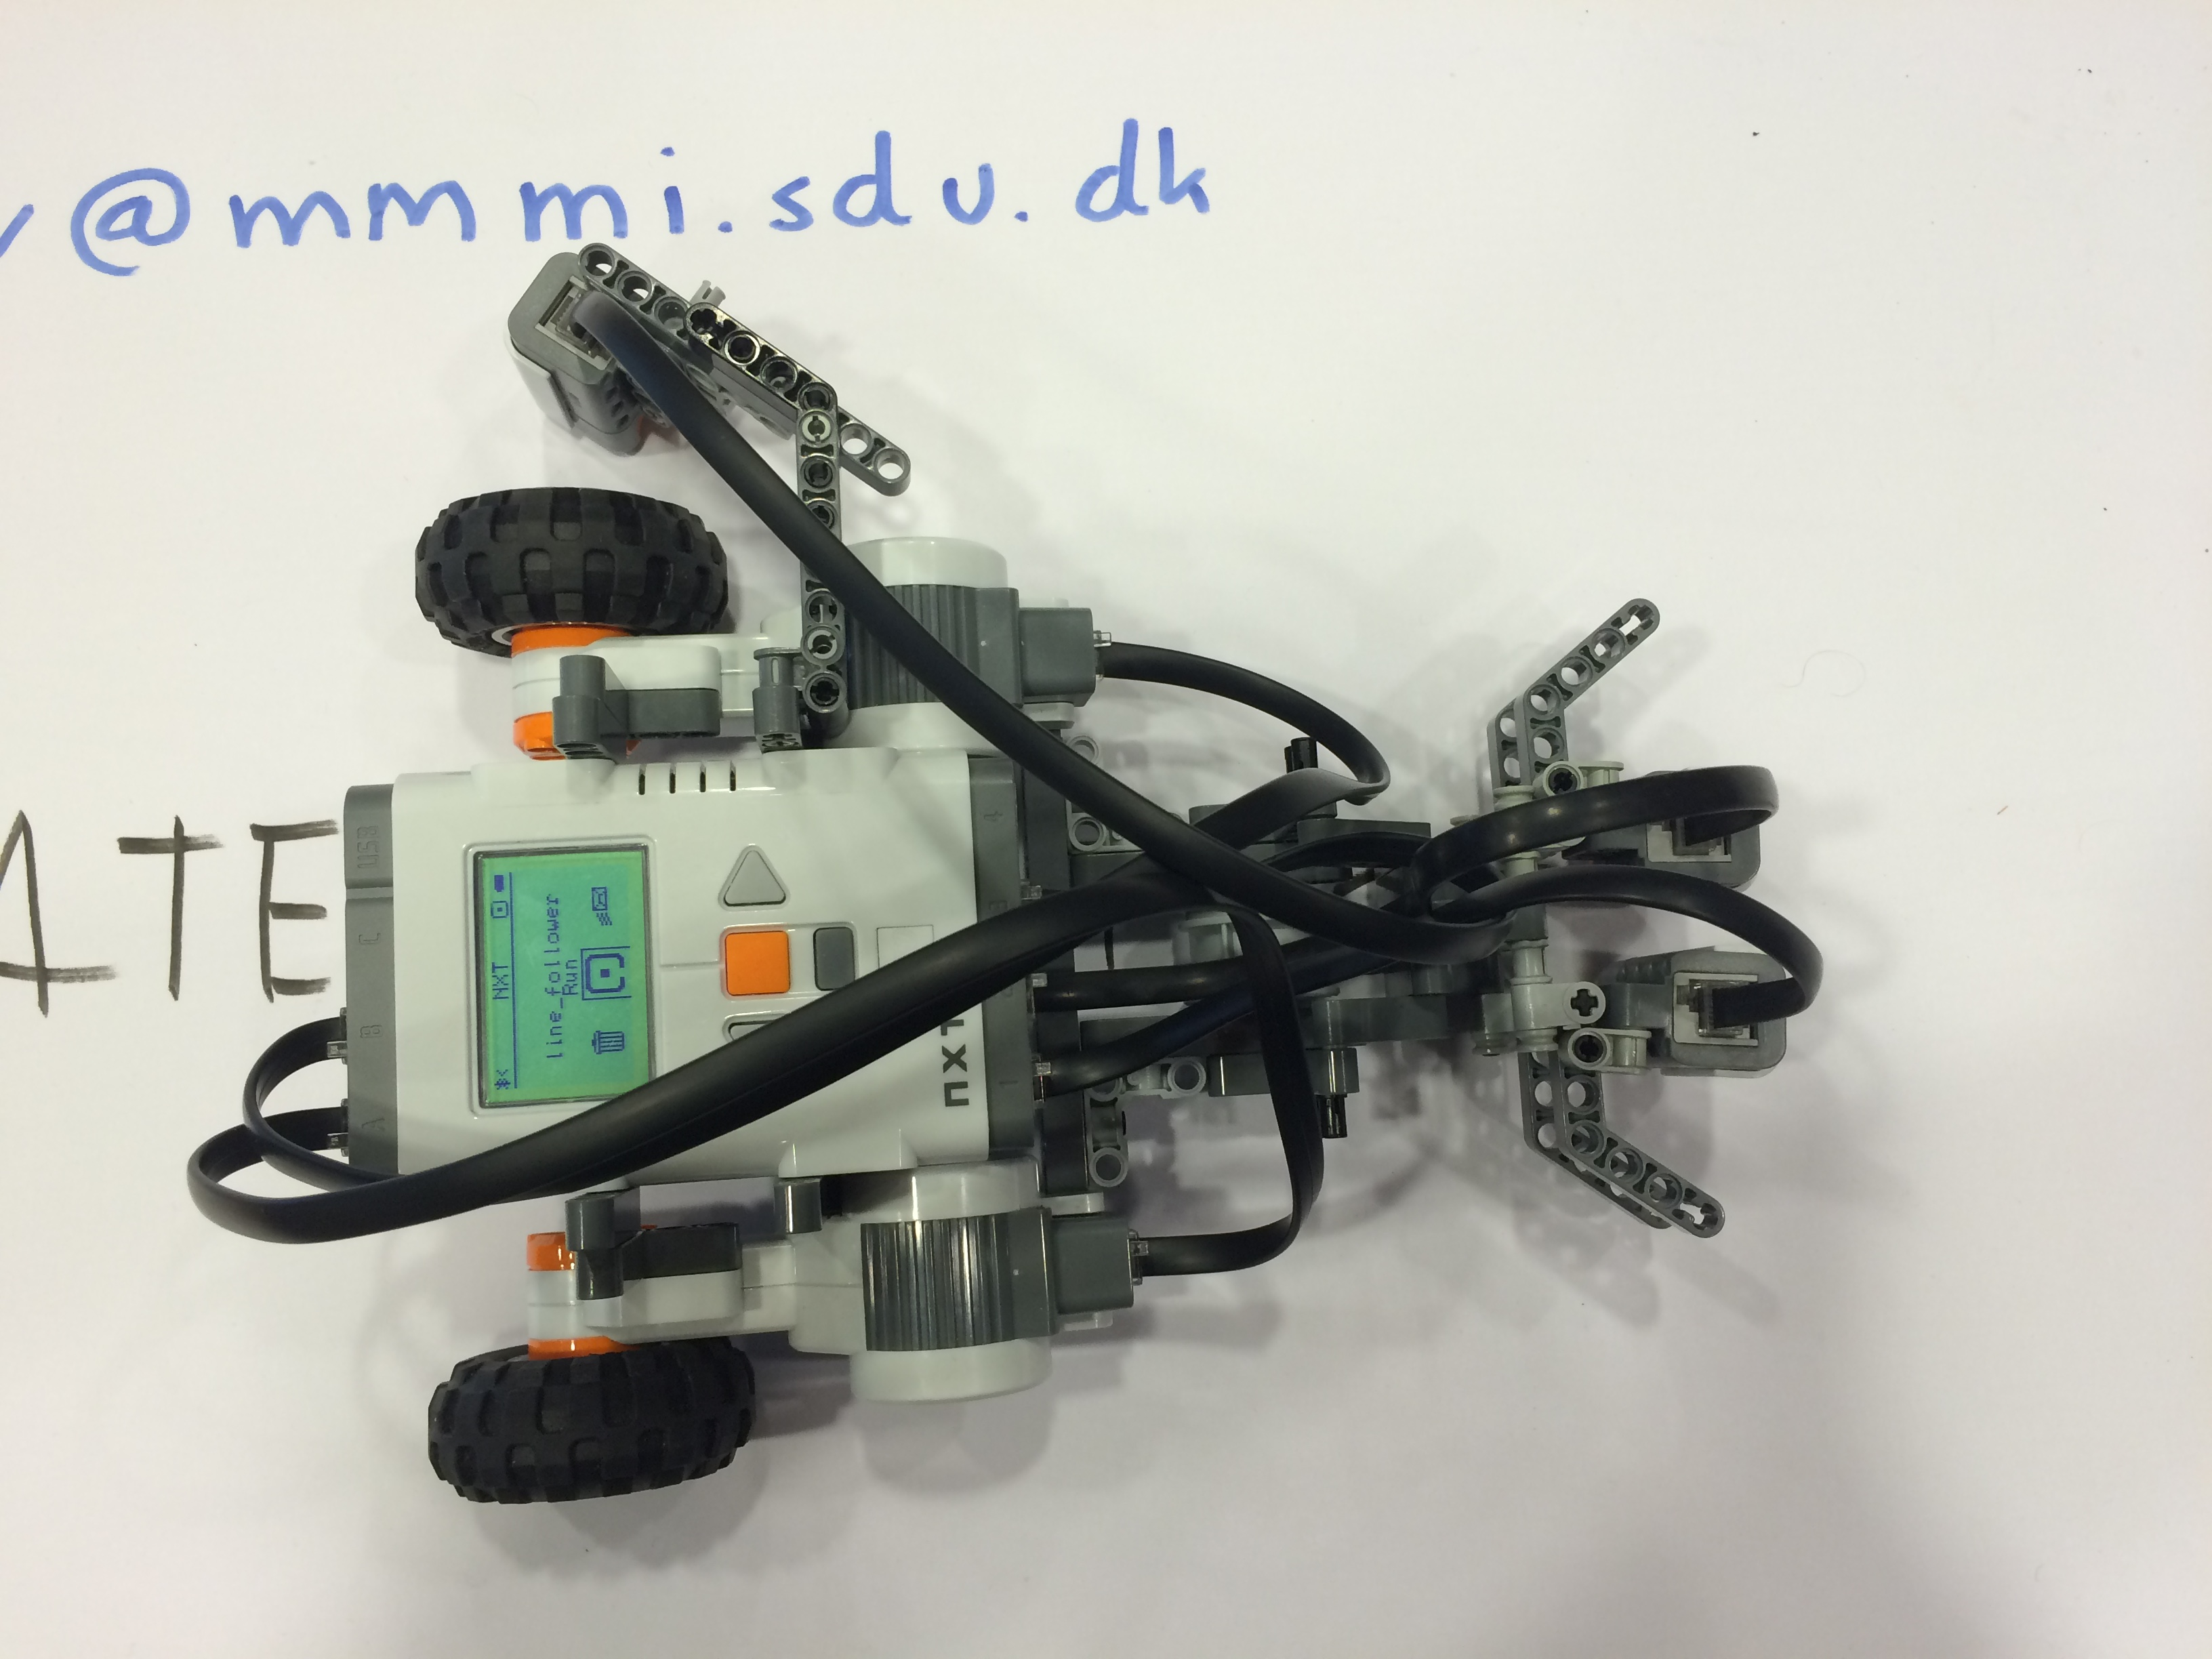
\includegraphics[width=\textwidth]{robot.jpg}
  \end{center}
  \caption{The current version of the robot}
\end{figure}   			

It has has been considered  whether the sensor in front should be moved to the back of the robot, such that the functionality of the sensors in the front does not get interrupted by the tin it pushes. \\


The line follower is done by computing the difference of the 2 front sensors.  If the difference between these two sensors are 0, that would mean both sensors are above the same color.    From different tests it could be seen that both sensors did not measure the same value, for which a bias value has been added to the difference such that the difference becomes zero when the both measure the same color.  It is at the moment not known whether if the bias value still would work for different lighting conditions.\\

The functions left() and right() only uses only the third sensor placed at the side of the robot, to either turn to the right or left,  which might create some problems if the sensor detect something darkish, not being the line.  If that occurs, the program continue the line following on white area, and keep moving until one of the sensors sees something black.\\\\
 
\textbf{3.  What factors do you think will affect the speed and reliability with which your
     robot can execute the Sokoban solution?  How will you evaluate and optimise them?
     (Or, will you optimise them, in fact?)}\\
     

		The speed at which the line follower moves has at level such that the line following still is reliable.   This value can only be found by testing the system at different speed levels, and observe it.\\
		
		As stated before is the the difference between both sensors computed using a bias value, whether this works for different is not known, which make is unreliable. An optimal solution would entail the sensor knowing the lighting condition and thereby adjust  the bias value accordingly.  Another way would be testing it at different lighting condition, and based from the test come up with an value that works. \\\\
		\textbf{4.  How will you test and document your robot
		's performance for the final report?}\\\\

The performance of the robot will be documented based on how reliably it performs the actions which is implemented onto it. \\


	The  functionality of the movements of the robot would be tested by giving it a string making move in eights.   It could be seen after a reasonable amount of iteration that the robot still followed the line, and was capable of correcting itself when   it was needed. \\
	
	The functionality of moving the tin but could be tested in the same manner as before, in which the robot is provided with a list which make the tin move in eights,  but would that require a bigger map. Another way testing this could be moving the tin in a square with different orientation, which would make it possible to test how precisely it moves the tin to next position. \\
	
	
	

	
	


\end{document}
